% Bleibende Regelabweichung: P-Regler am Füllprozess mit offenem Ventil (P04 A3)
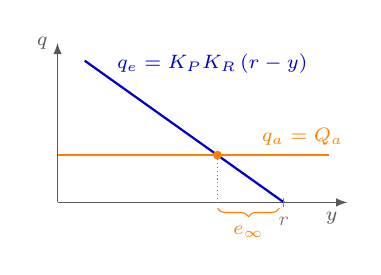
\begin{tikzpicture}[x=1.15cm,y=0.75cm,font=\scriptsize]
	\draw[-latex,gray!70!black] (0,0) -- (3.2,0) node[below left] {$y$};
	\draw[-latex,gray!70!black] (0,0) -- (0,2.7) node[left] {$q$};
	\draw[blue!80!black, thick] (0.3,2.4) -- (2.5,0);
	\node[blue!80!black, anchor=west] at (0.55,2.35) {$q_e = K_P K_R\,(r-y)$};
	\draw[orange, thick] (0,0.8) -- (3.0,0.8);
	\node[orange, anchor=south west] at (2.15,0.8) {$q_a = Q_a$};
	\fill[orange] (1.767,0.8) circle (1.6pt);
	\draw[gray, densely dotted] (1.767,0.8) -- (1.767,0);
	\draw[gray] (2.5,0.08) -- (2.5,-0.08) node[below] {$r$};
	\draw[orange, decorate, decoration={brace,mirror,amplitude=3pt}]
		(1.767,-0.1) -- (2.45,-0.1) node[midway,below=3pt] {$e_\infty$};
\end{tikzpicture}
